%!TEX root = ../rapport.tex

\section{Conception}
\label{section:conception_client}
La section ci-dessous a comme objectif de mettre en avant les choix de conception pour l'application. Premièrement, des maquettes seront présentées. Ensuite, l'architecture sera expliqué au travers du \emph{Storyboard} et des différentes contrôlleurs qui composent l'application. Finalement, les entités de l'application ont été schématisées et détaillées.

\subsection{Maquettes} % (fold)
\label{sub:maquettes}

Ci-dessous les maquettes créées permettent de se donner une meilleure idée sur le visuel de l'application finale. Sauf contraintes techniques, l'application ressemblera, à quelques exceptions près, le plus possible à ces mauqettes.

\subsubsection{Authentification}
La figure \ref{gra:maqLogin} montre comment sera présentera l'écran qui permettra de s'authentifier pour entrer dans l'application. L'utilisateur entre son login et son mot de passe et clique sur le bouton login. Dans le cas où les informations sont fausses ou si quelque choses s'est mal passé, un message lui sera proposé.
\begin{figure}[H]
      \centering
      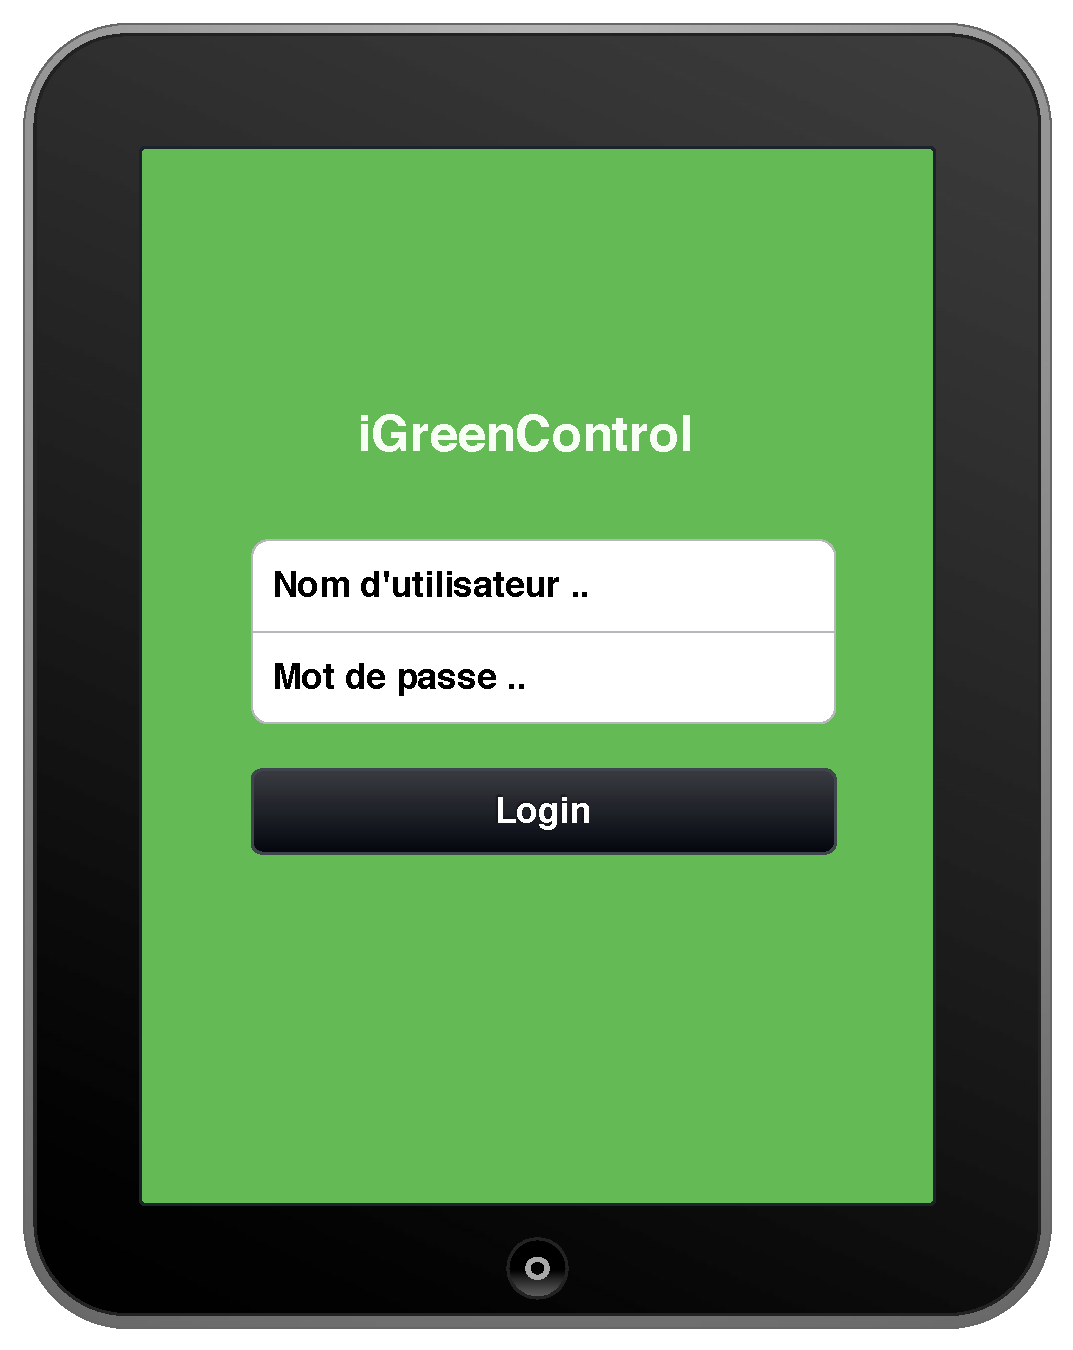
\includegraphics[width=8cm]{00_media/04_Maquette_00.pdf}
      \caption{Maquette - Login}
      \label{gra:maqLogin}
\end{figure}
\subsubsection{Menu général}
La figure \ref{gra:maqmenu} représente le menu de l'application. Celui-ci est composé de 6 boutons. Ci-dessous une description de ce qui est possible de faire avec chaque bouton.

\medskip

\begin{itemize}
  \item Le bouton \textbf{Maison} permet de lister les maisons dans le but d'en ouvrir une spécifique ou d'en créer une nouvelle
  \item Le bouton \textbf{Sauver} permet de sauver la maison en cours d'édition
  \item Le bouton \textbf{Importer plan} permet de choisir une image dans la librairie des photos de l'\emph{\gls{ipad}}.
  \item Le bouton \textbf{Insérer zone} permet d'insérer une nouvelle zone sur le plan ouvert
  \item Le bouton \textbf{Logout} permet de se déloguer et ainsi d'arriver à nouveau sur l'écran représenté par la figure \ref{gra:maqLogin} 
  \item Le bouton   \textbf{Infos} permet de voir des informations propres à l'application
\end{itemize}
\begin{figure}[H]
      \centering
      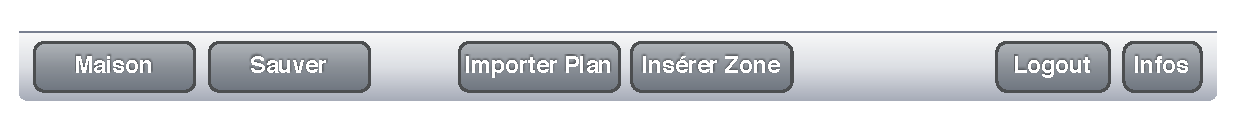
\includegraphics[width=\textwidth]{00_media/04_Maquette_Menu.pdf}
      \caption{Maquette - Menu}
      \label{gra:maqmenu}
\end{figure}
\subsubsection{Menu pour les maisons}
La figure \ref{gra:maq01} sera l'écran visible quand l'utilisateur cliquera sur le bouton \textbf{Maison}. Il peut alors soit ouvrir une maison, soit créer une nouvelle maison.
\begin{figure}[H]
      \centering
      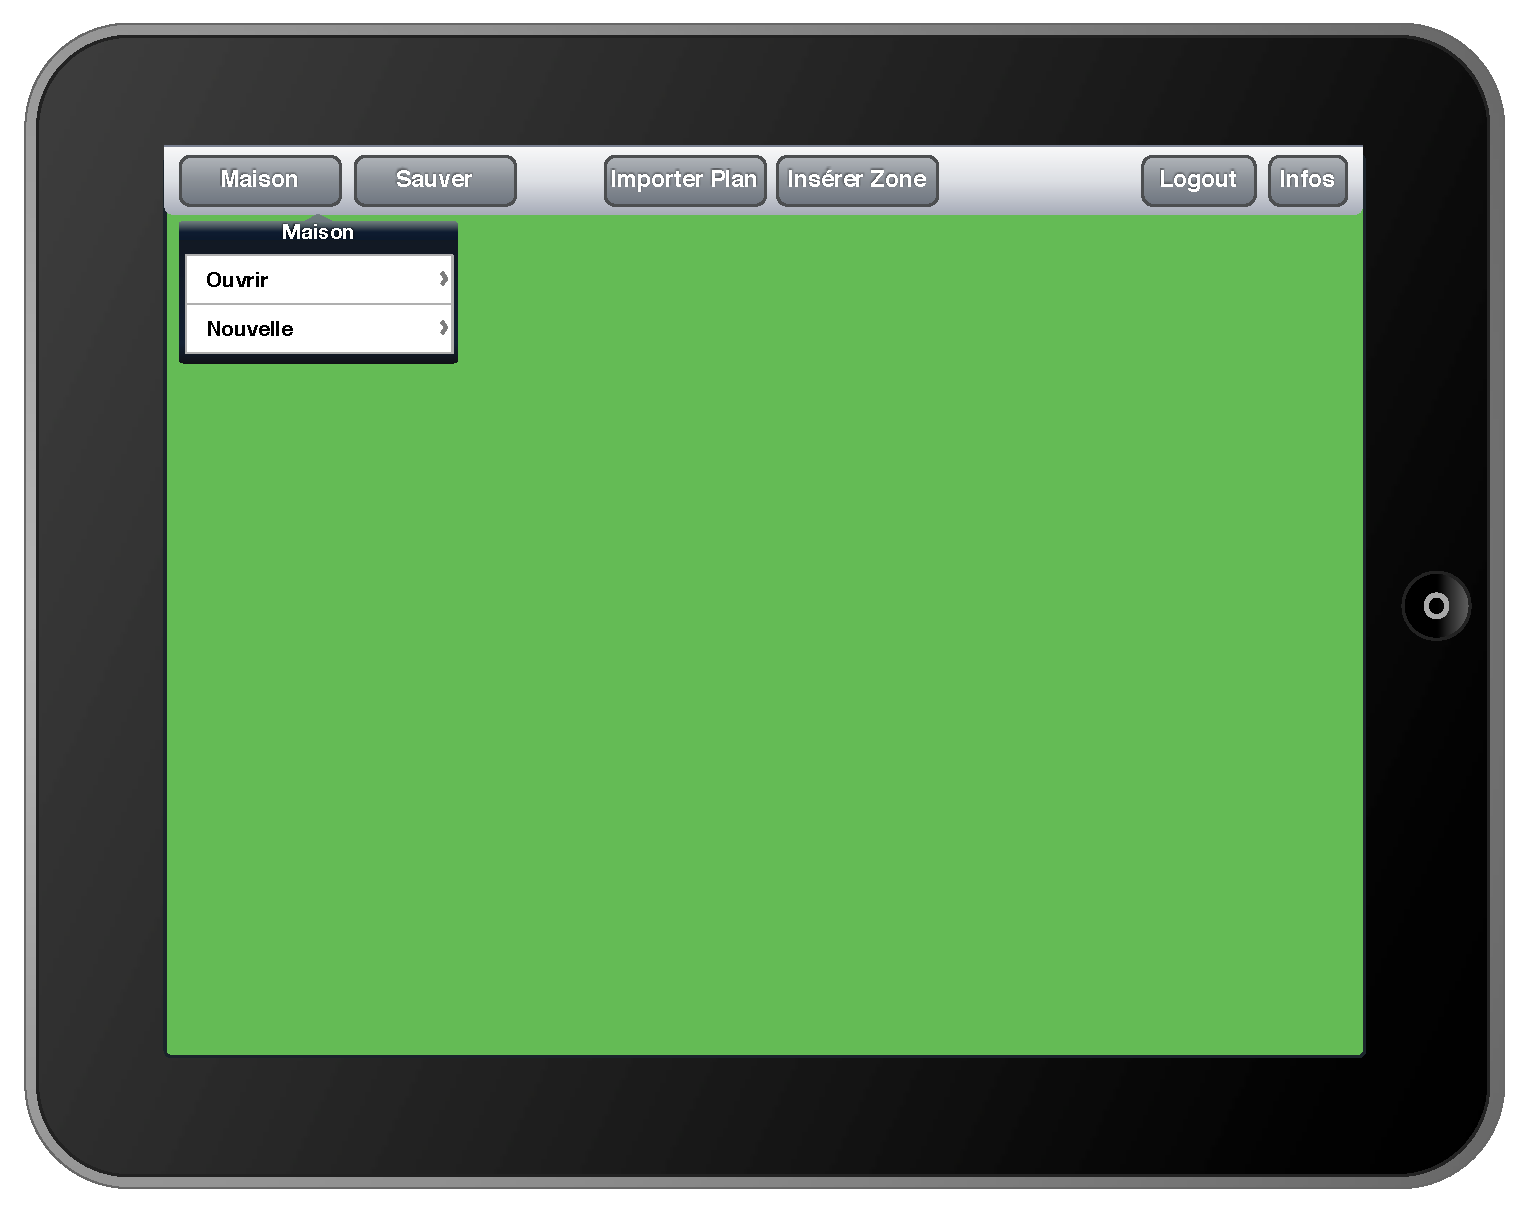
\includegraphics[width=9cm]{00_media/04_Maquette_01.pdf}
      \caption{Maquette - Menu Maison}
      \label{gra:maq01}
\end{figure}
\subsubsection{Lister les maisons}
La figure \ref{gra:maq02} propose la liste des maisons qui sont concernées par l'utilisateur loggué. S'il clique sur une maison, celle-ci s'ouvre dans l'application.

\medskip

Il peut également afficher le bouton pour supprimer une maison en passant son doigt de gauche à droite sur la maison.

\medskip

Un champ de recherche sera également présent dans le cas où l'utilisateur a beaucoup de maison et qu'il souhaite en rechercher une particulière.

\begin{figure}[H]
      \centering
      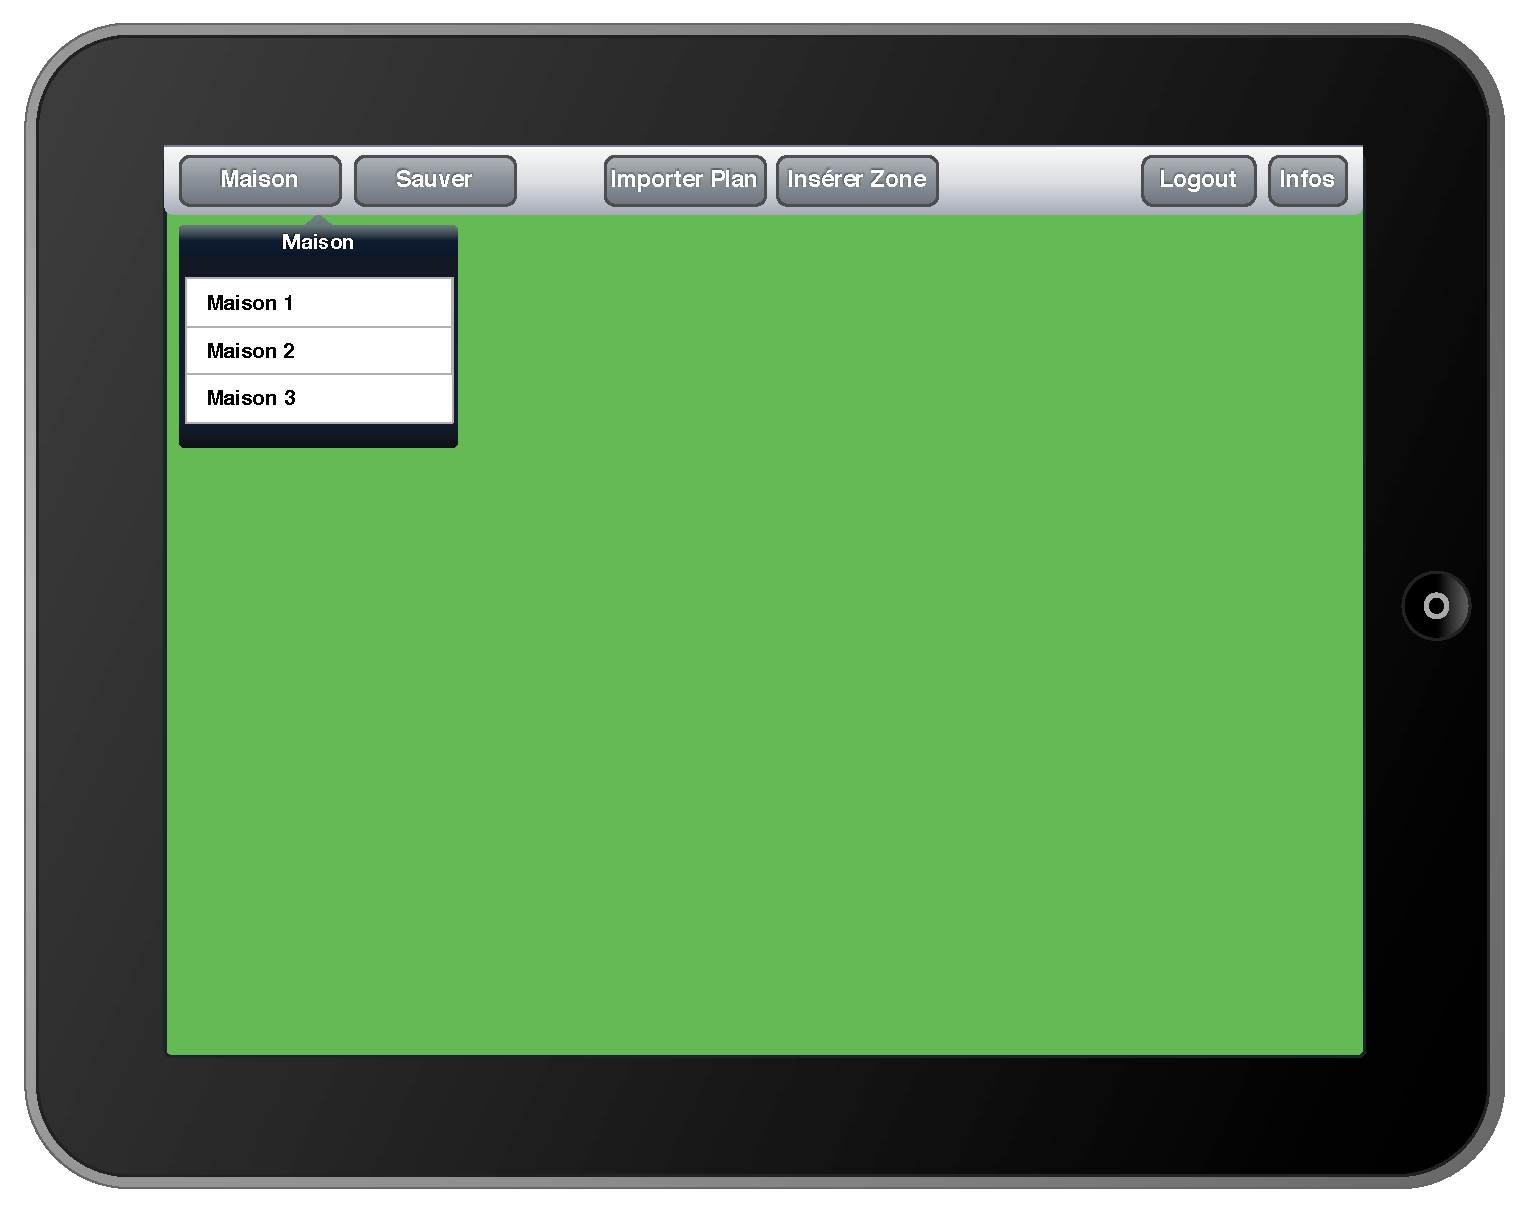
\includegraphics[width=9cm]{00_media/04_Maquette_02.pdf}
      \caption{Maquette - Liste Maison}
      \label{gra:maq02}
\end{figure}
\subsubsection{Créer une nouvelle maison}
La figure \ref{gra:maq03} apparaît si l'utilisateur clique sur nouvelle maison. Il doit alors entrer les informations qui sont utiles à la création de la maison puis cliquer sur le bouton pour sauvegarder la maison.
\begin{figure}[H]
      \centering
      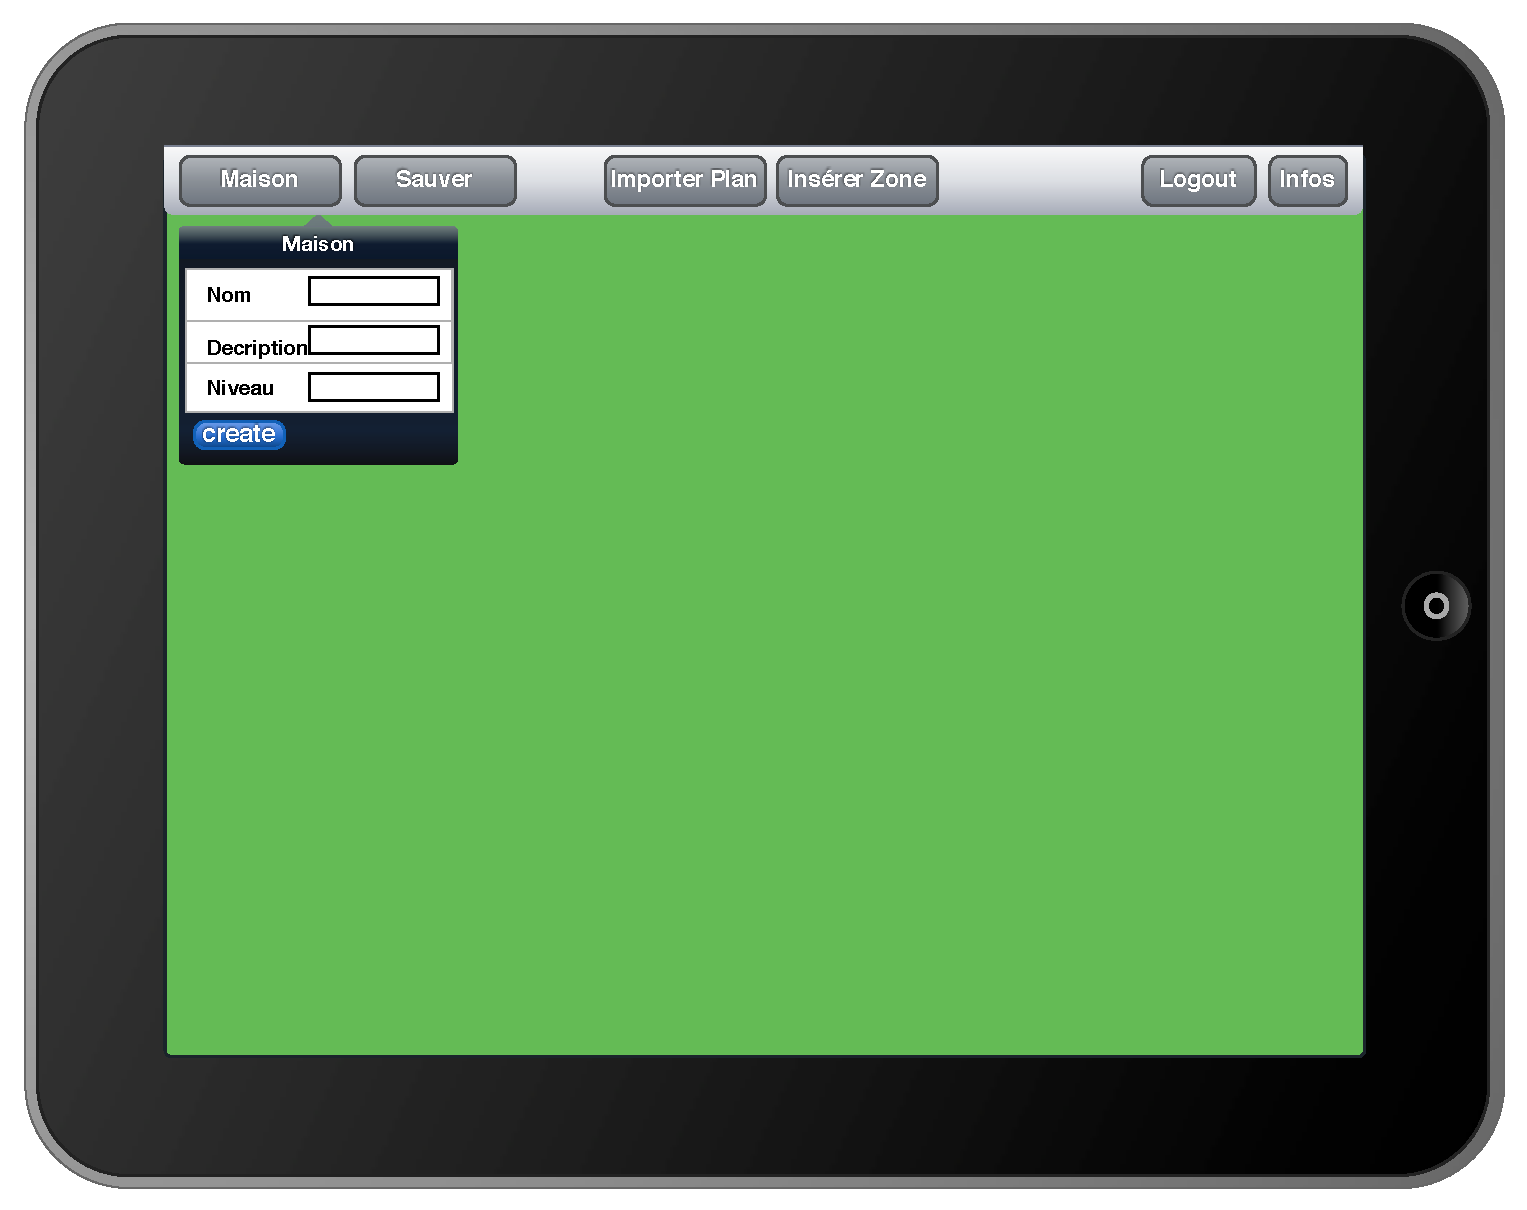
\includegraphics[width=9cm]{00_media/04_Maquette_03.pdf}
      \caption{Maquette - Nouvelle Maison}
      \label{gra:maq03}
\end{figure}
\subsubsection{Enregistrer une maison}
La figure \ref{gra:maq04} apparaît si l'utilisateur désire sauver la maison en cours. Il doit alors entrer les informations qu'il désire modifié puis cliquer sur le bouton pour sauvegarder la maison. Toutes les modifications effectuées seront alors sauvées.
\begin{figure}[H]
      \centering
      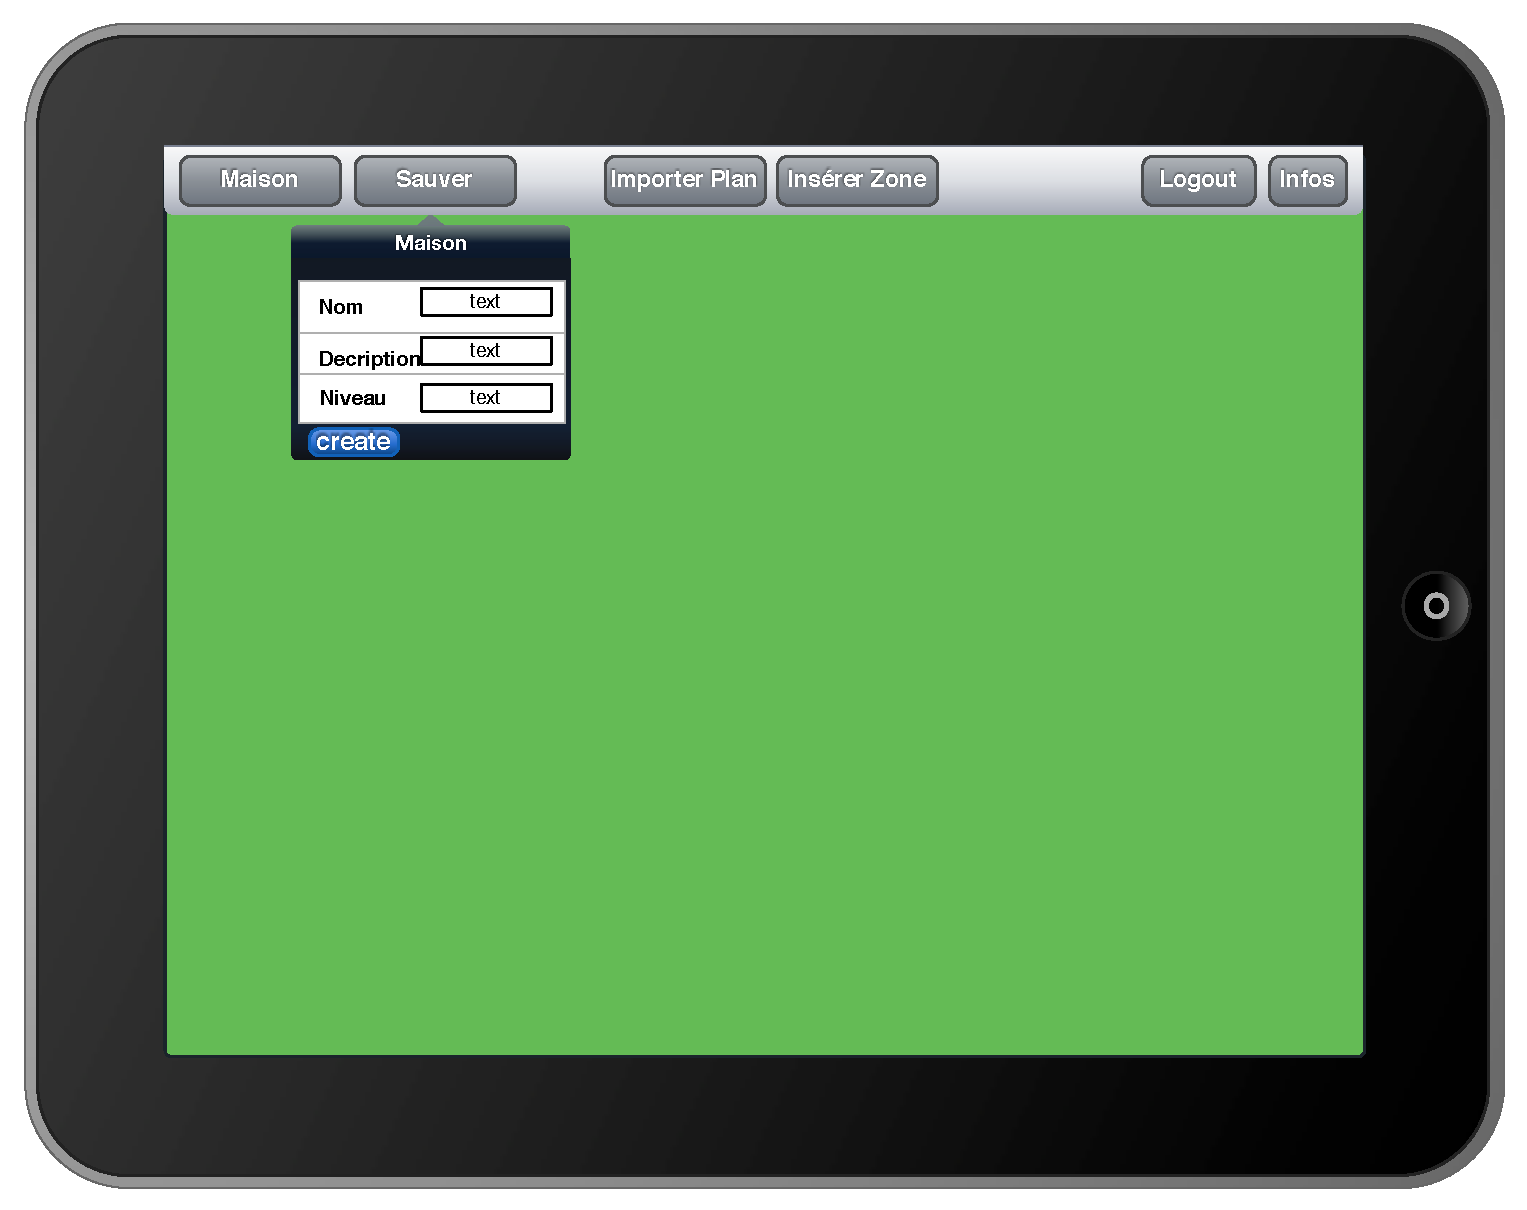
\includegraphics[width=9cm]{00_media/04_Maquette_04.pdf}
      \caption{Maquette - Sauver Maison}
      \label{gra:maq04}
\end{figure}
\subsubsection{Import d'une image}
La figure \ref{gra:maq05} intervient lorsque l'utilisateur veut importer un plan. Un explorateur d'images apparaît et il peut rechercher une photo qui est présente dans sa librairie de photos.
\begin{figure}[H]
      \centering
      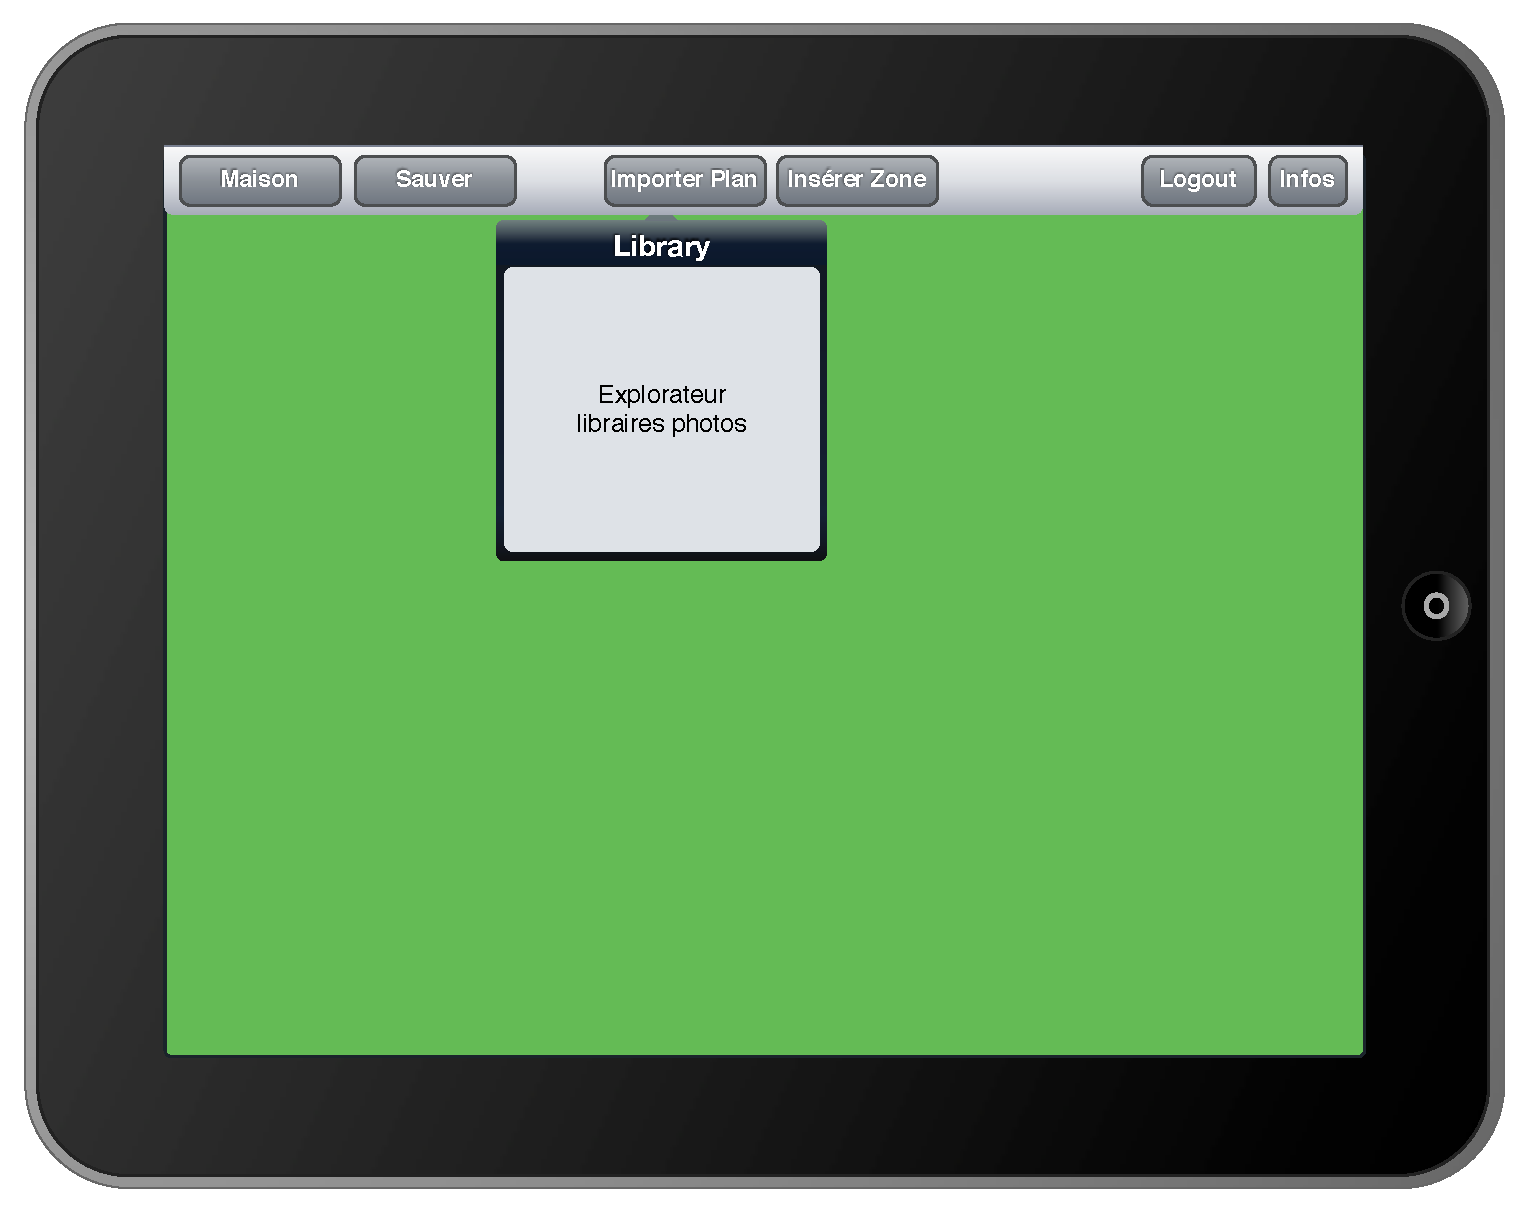
\includegraphics[width=9cm]{00_media/04_Maquette_05.pdf}
      \caption{Maquette - Import image}
      \label{gra:maq05}
\end{figure}
\subsubsection{Affichage du plan}
Quand une image a été selectionnée, celle-ci vient se position sur l'écran comme le montre la figure \ref{gra:maq06}. L'utilisateur pourra en modifier la position et la taille grâce à tes reconnaissances de gestes.
\begin{figure}[H]
      \centering
      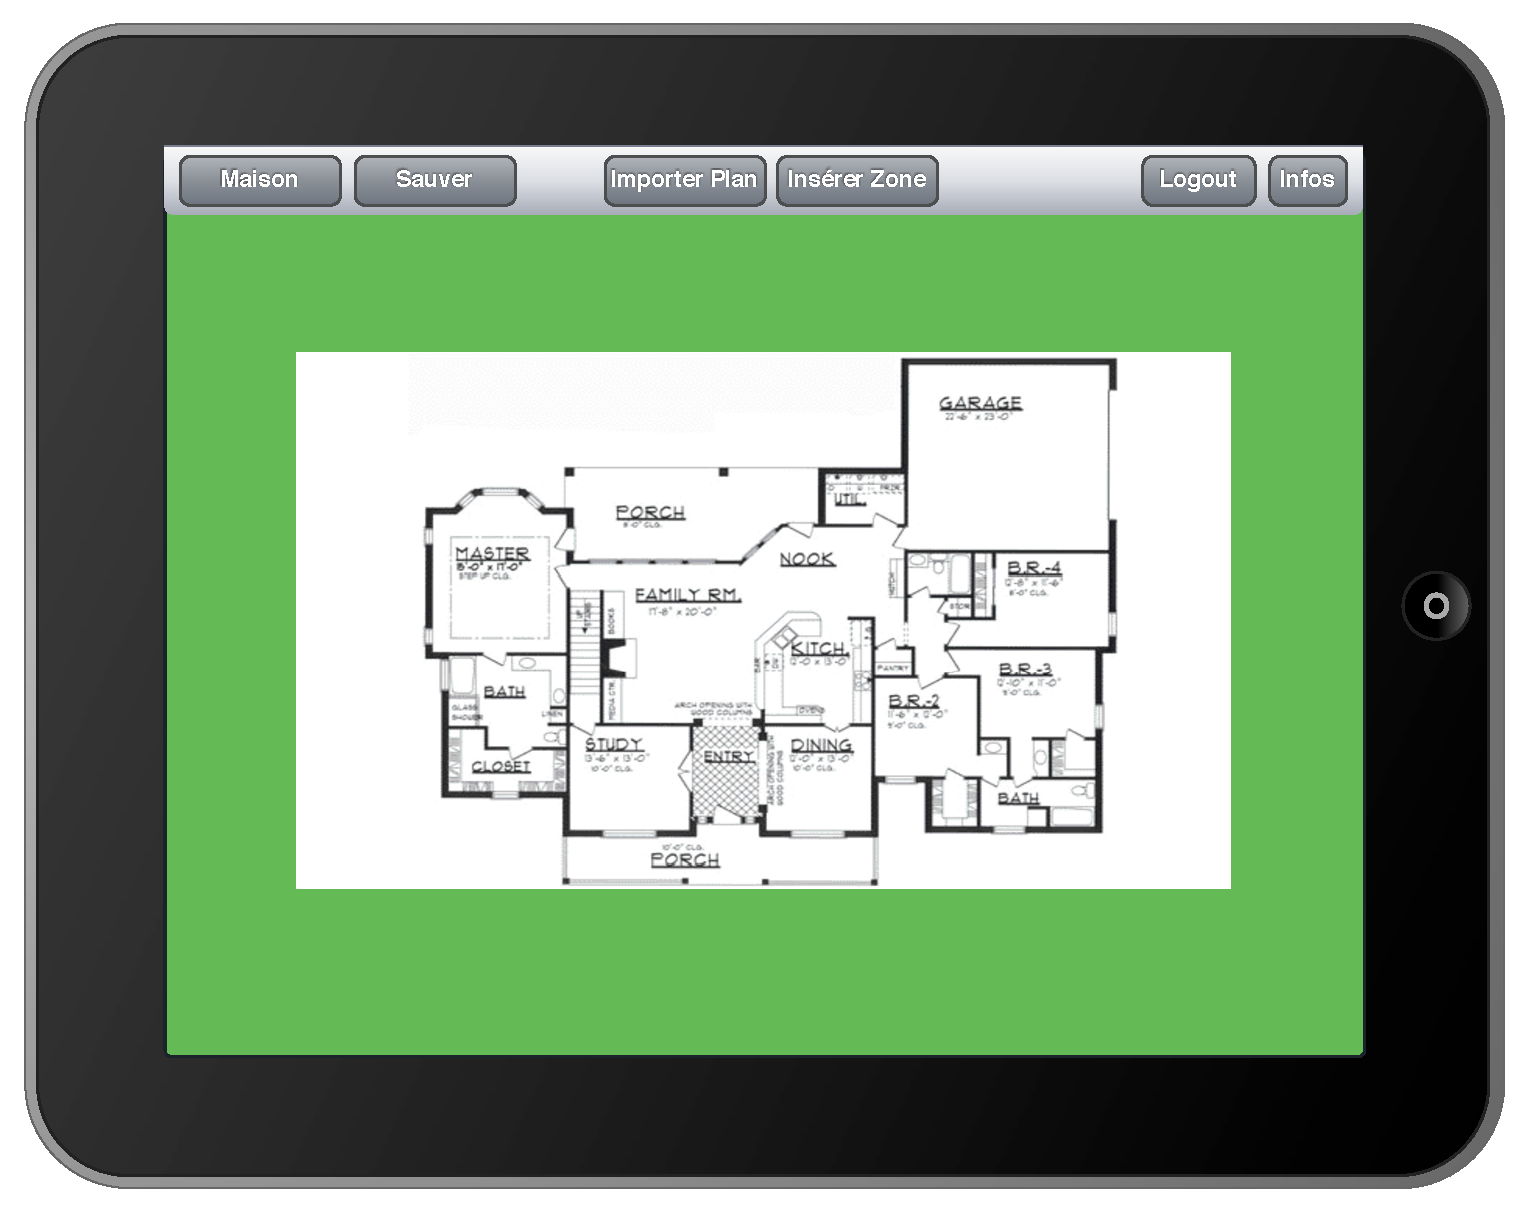
\includegraphics[width=9cm]{00_media/04_Maquette_06.pdf}
      \caption{Maquette - Plan}
      \label{gra:maq06}
\end{figure}
\subsubsection{Insertion d'une nouvelle zone}
Lorsque l'utilisateur veut insérer une nouvelle zone, il doit entrer des paramètres correspondant à la zone puis cliquer sur le bouton comme le montre la figure \ref{gra:maq07}.
\begin{figure}[H]
      \centering
      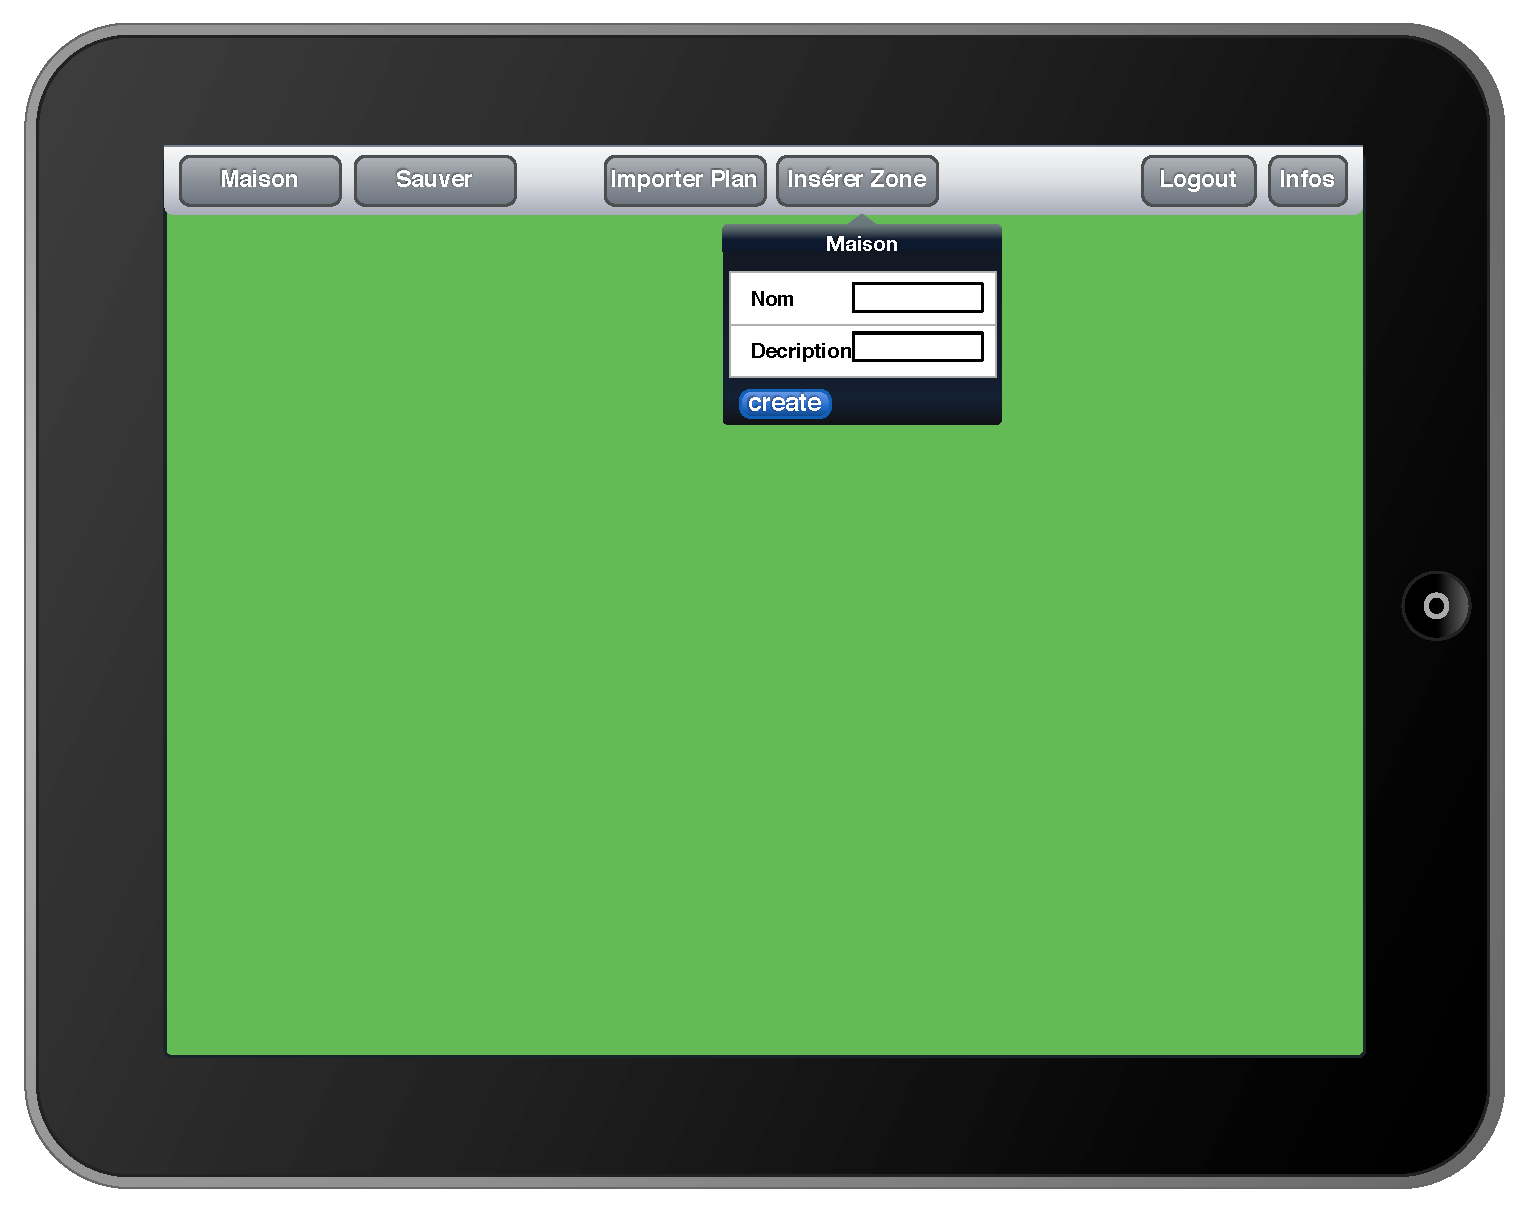
\includegraphics[width=9cm]{00_media/04_Maquette_07.pdf}
      \caption{Maquette - Nouvelle zone}
      \label{gra:maq07}
\end{figure}
\subsubsection{Représentation des zones}
Lorsque la zone a été insérée, elle peut être visible par un rectangle sur le plan comme le montre la figure \ref{gra:maq08}. La zone peut être redimensionnée ou déplacée. On peut même la faire pivoter grâce à des reconnaissances de gestes.

\begin{figure}[H]
      \centering
      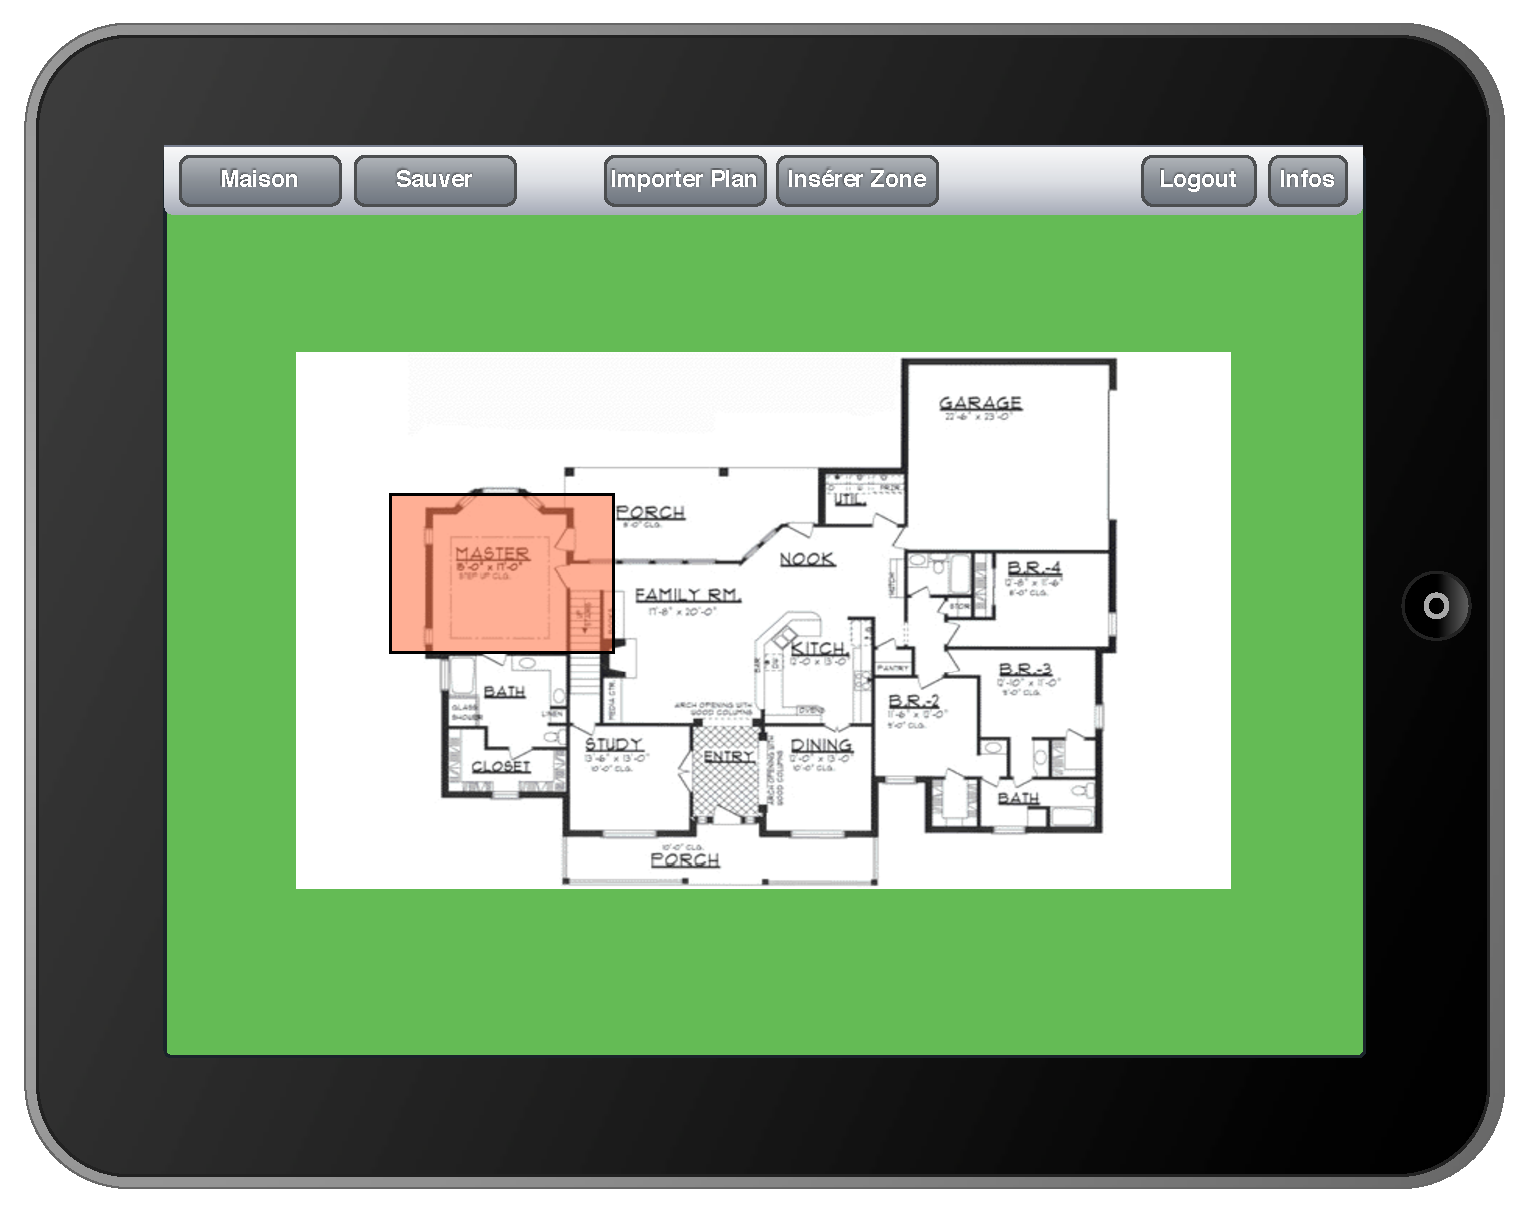
\includegraphics[width=9cm]{00_media/04_Maquette_08.pdf}
      \caption{Maquette - Zone}
      \label{gra:maq08}
\end{figure}
\subsubsection{Options sur les zones}
Lorsque l'utilisateur presse un certain moment sur une zone, un menu apparaît comme sur la figure \ref{gra:maq09}. Il peut alors modifier les paramètres de la zone comme le nom, la description et d'autres informations. Il peut également supprimer la zone ou insérer un capteur dans la zone.
\begin{figure}[H]
      \centering
      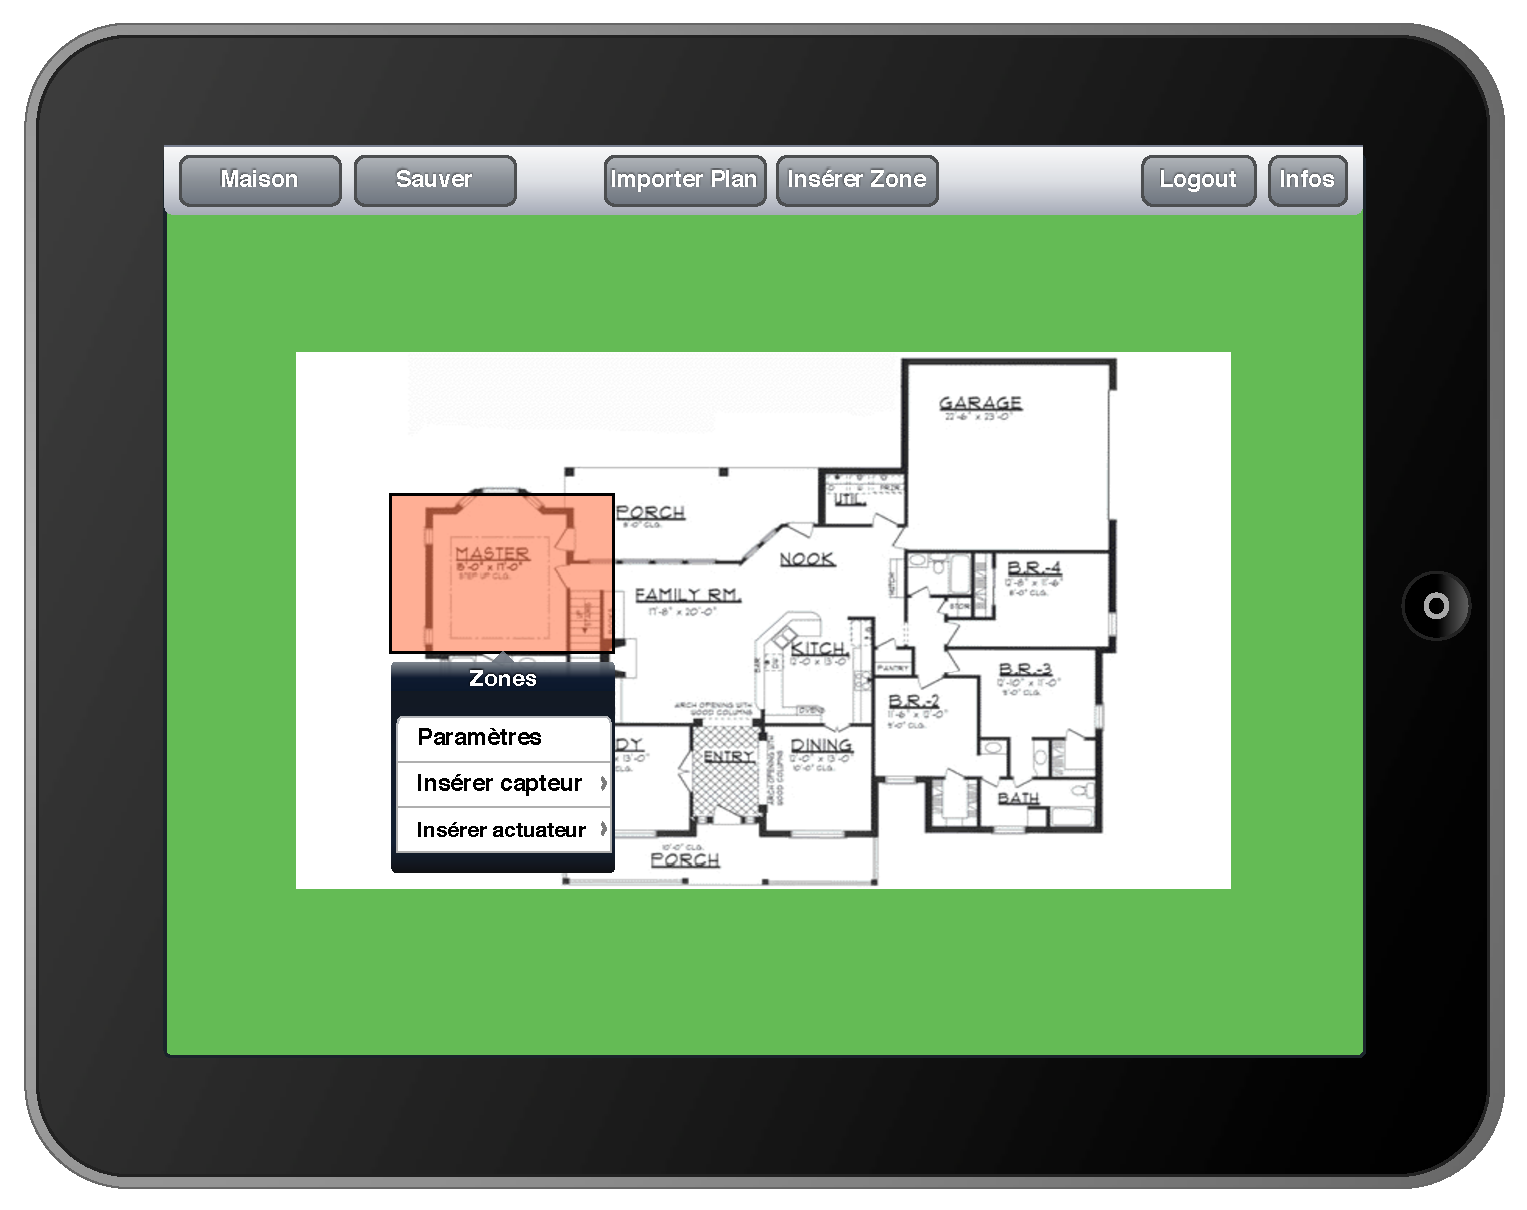
\includegraphics[width=9cm]{00_media/04_Maquette_09.pdf}
      \caption{Maquette - Options sur une zone}
      \label{gra:maq09}
\end{figure}
\subsubsection{Représentation des capteurs}
Lorsqu'un capteur est inséré, il est représenté directement dans la zone correspondante. Le rectangle bleu de la figure \ref{gra:maq10} représente un capteur.
\begin{figure}[H]
      \centering
      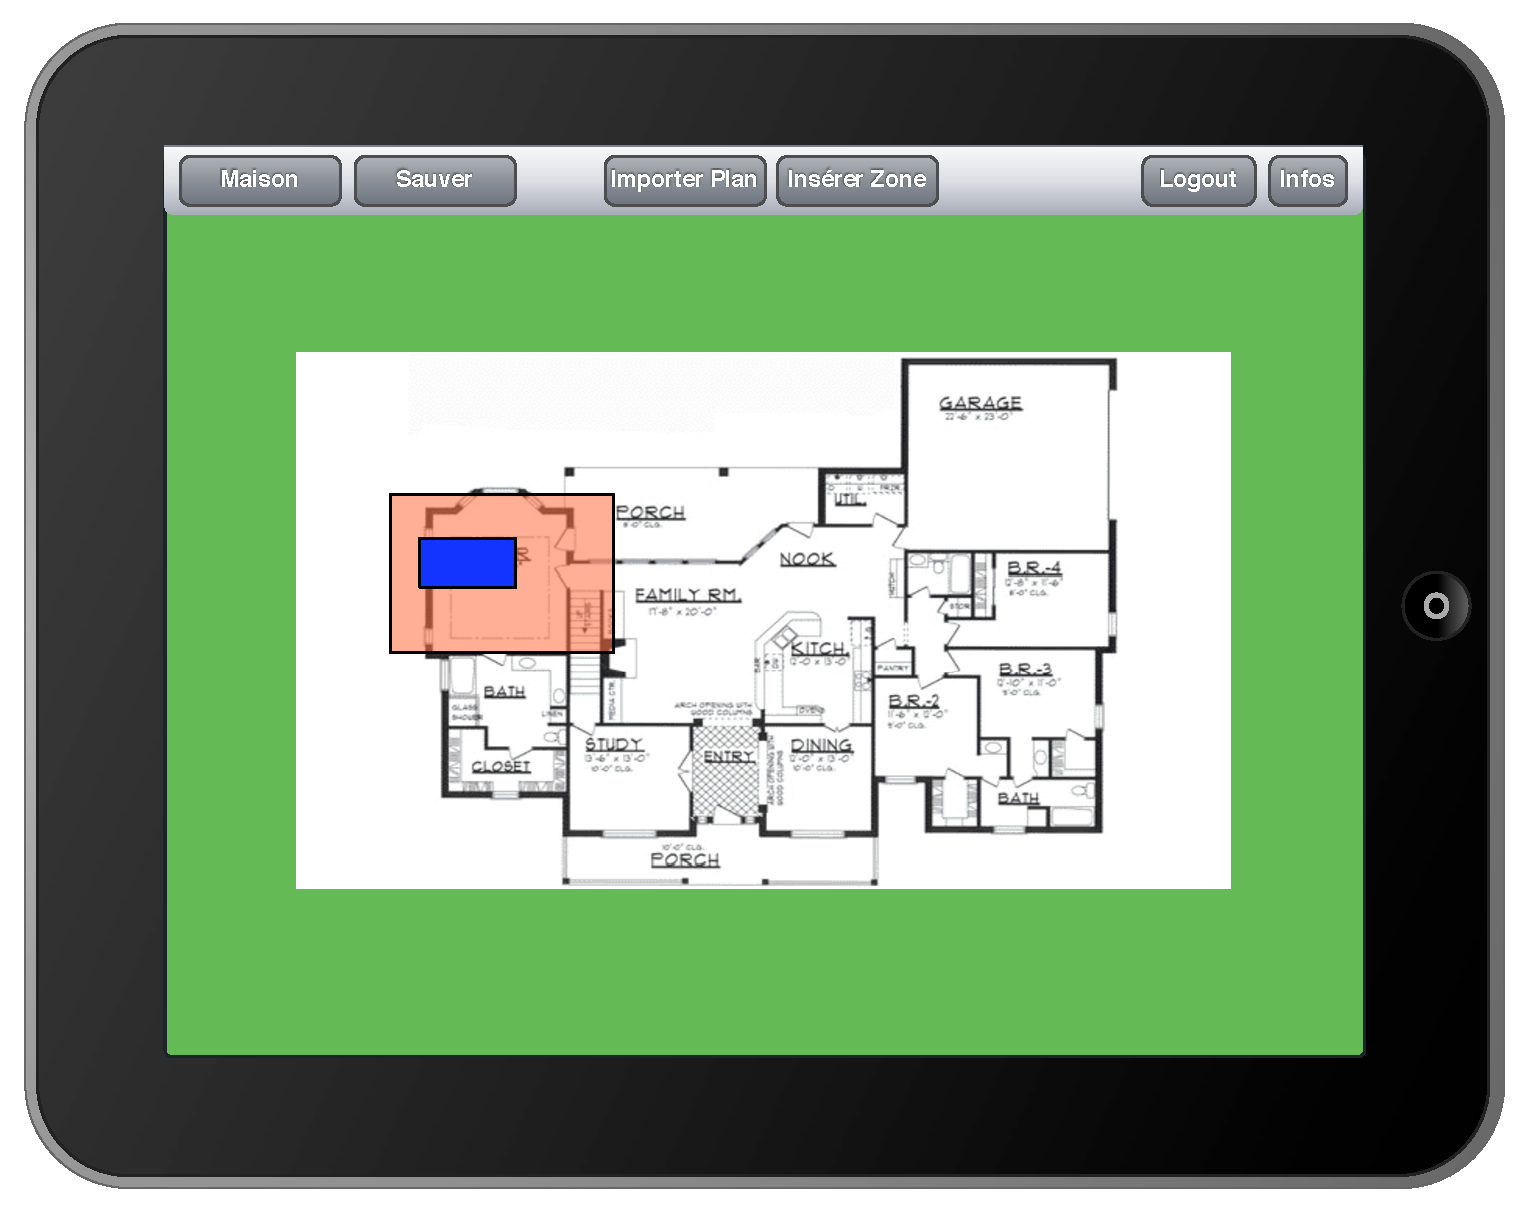
\includegraphics[width=9cm]{00_media/04_Maquette_10.pdf}
      \caption{Maquette - Capteur}
      \label{gra:maq10}
\end{figure}
\subsubsection{Options sur les capteurs}
Lorsque l'utilisateur presse un certain temps sur un capteur, un menu apparaît et permet d'effectuer des opération sur le capteur correspondant. Ceci est représenté par la figure \ref{gra:maq11}. Il peut le supprimer, en modifier les paramètres ou voir les données du capteur.
\begin{figure}[H]
      \centering
      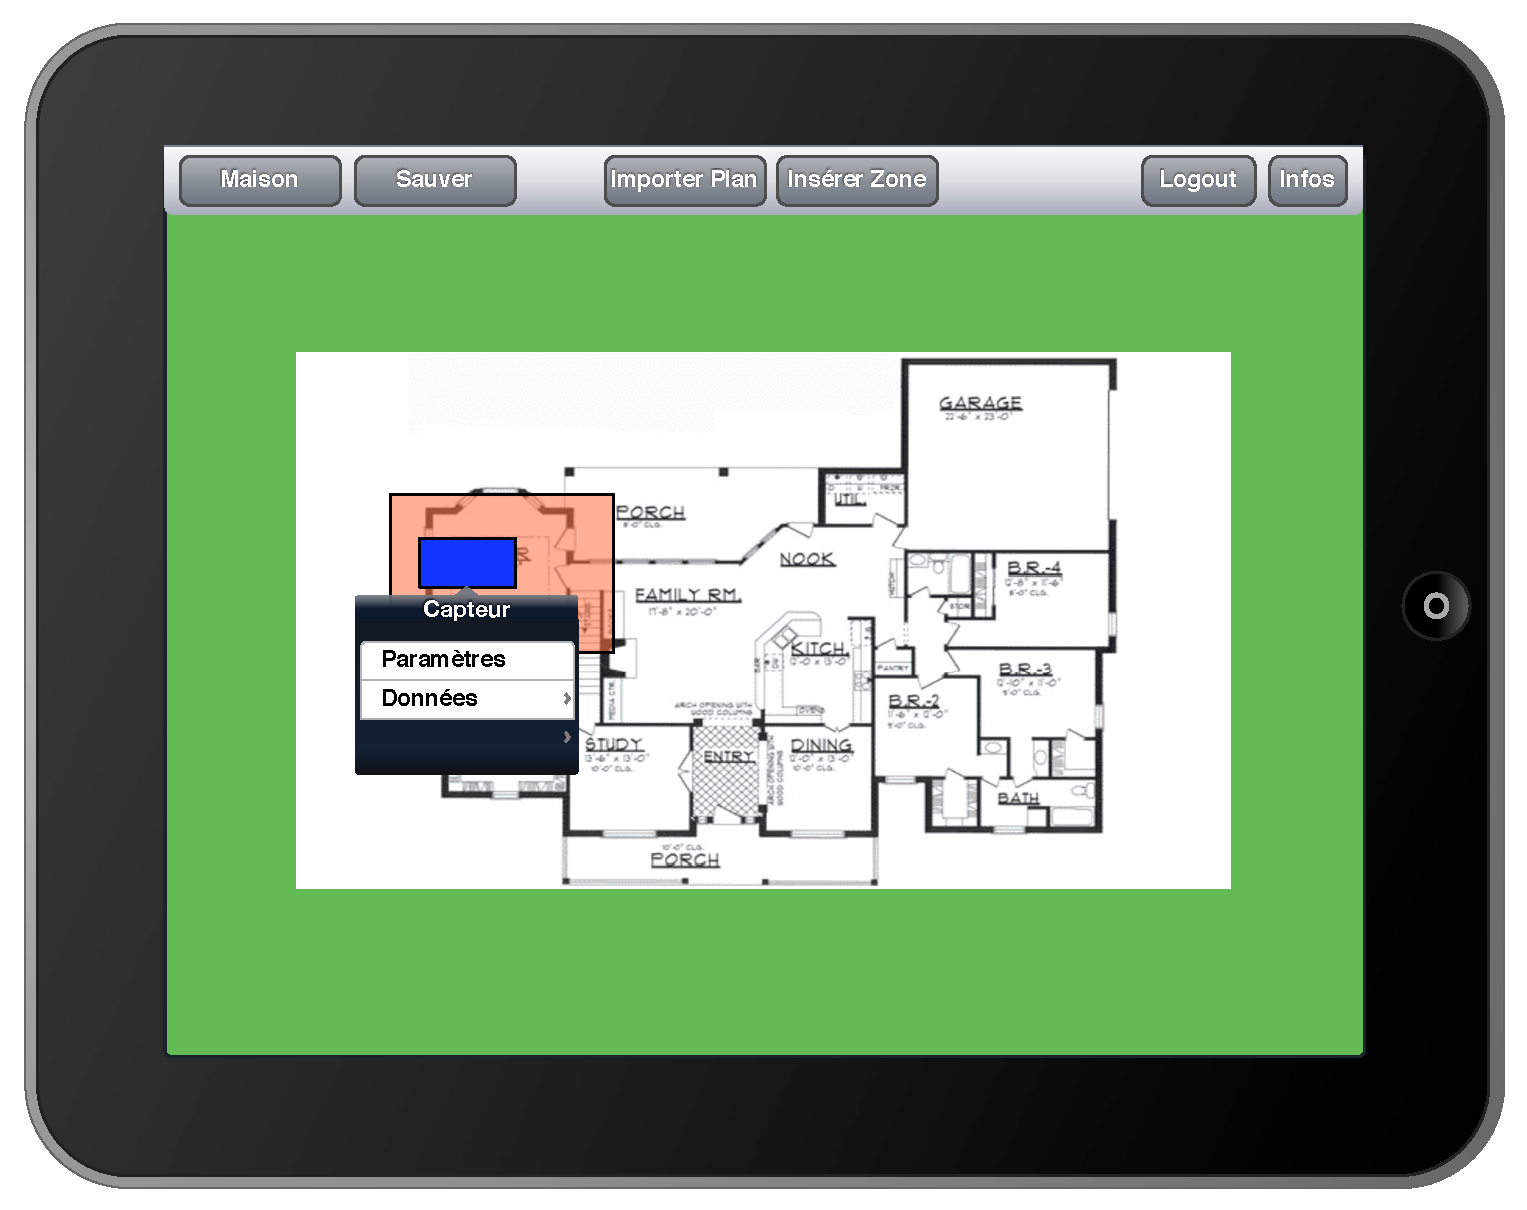
\includegraphics[width=9cm]{00_media/04_Maquette_11.pdf}
      \caption{Maquette - Options sur capteur}
      \label{gra:maq11}
\end{figure}
\subsubsection{Informations sur l'application}
La figure \ref{gra:maq12} montre le \emph{About} de l'application. L'utilisateur pourra lire des informations relatives à l'application.
\begin{figure}[H]
      \centering
      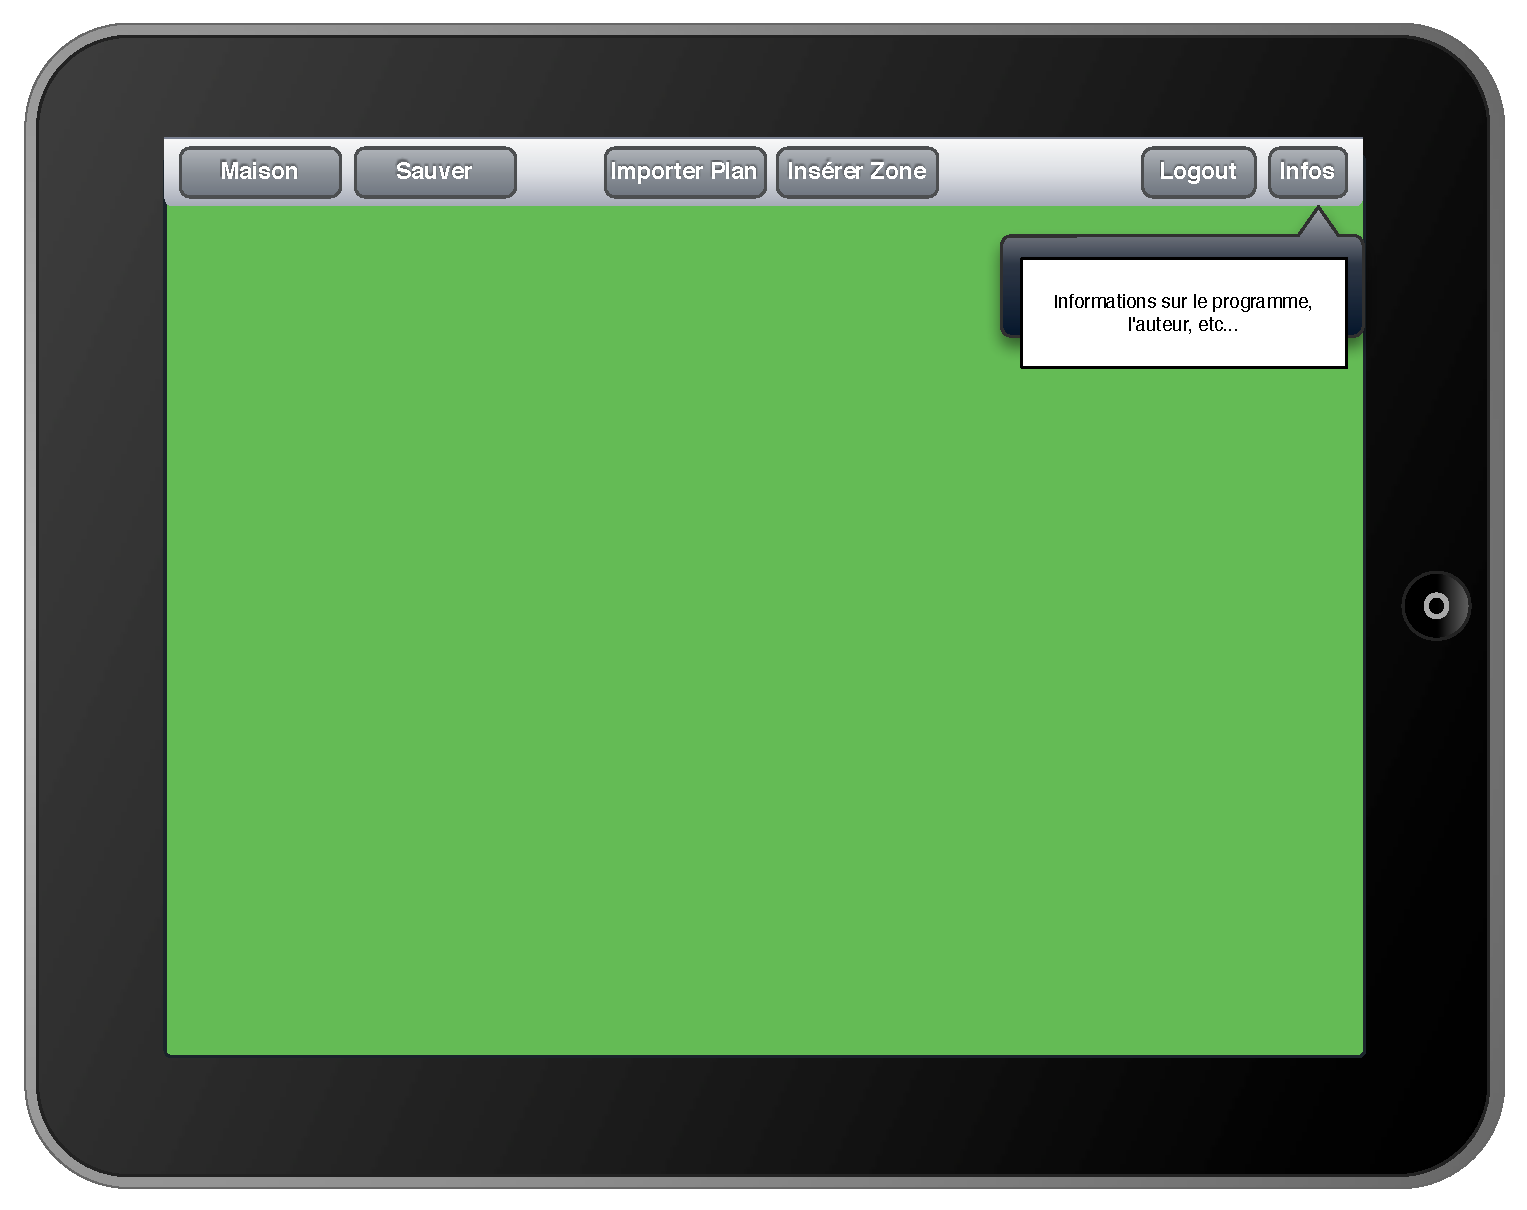
\includegraphics[width=9cm]{00_media/04_Maquette_12.pdf}
      \caption{Maquette - Infos}
      \label{gra:maq12}
\end{figure}

\subsubsection{Supprimer les maisons}

Afin de supprimer les maisons, il suffira de faire un défilement de gauche à droite sur la maison désirée se trouvant dans la liste. Un bouton "supprimer" apparaîtra alors.

\subsection{Mode paysage / portrait}
L'application sera conçue pour être utiliser en mode paysage. Le seul écran qui pourra être en mode paysage et portrait est lorsque l'utilisateur veut se logguer.

\subsection{Architectures de l'application} % (fold)
\label{sub:architectures_de_l_application}

L'application a été découpé en 3 parties bien distinctes.

\medskip

\begin{itemize}
  \item Un dossier \emph{Model} regroupe les entités de l'application (User, House, Zone, Sensor, SensorData)
  \item Un dossier \emph{Controller} regroupe tous les contrôleurs de l'application
  \item Un dossier \emph{Delegate} regroupe tous les delegate de l'application
\end{itemize}

% subsection architectures_des_c (end)

\subsection{Architecture des contrôleurs} % (fold)
\label{sub:architecture_de_l_application}
Les contrôleurs permettent en résumé d'afficher les vues de l'application

\medskip

La figure \ref{gra:iGreencontrolStoryboard} représente le \emph{Storyboard} de l'application. En guise d'explicatif de l'architecture de l'application, je vais détailler ici comment les différentes vues ont été conçues.

\medskip

Le première écran, le login, est un contrôleur de type \emph{UIViewController}.

\medskip

L'écran principal de l'application, celui ou sera affiché les plans, les zones, etc.. est un contrôleur de type \emph{UIViewController}.

\medskip

Le contrôleur qui englobe le menu qui permet de gérer la liste des maisons et d'en créer est un \emph{UINavigationController} qui permet notamment de faire des transitions entre différents contrôleurs. C'est d'ailleurs pour cela que j'ai utilisé ceci puisque le menu, le formulaire pour créer une nouvelle maison et la liste des maisons sont des \emph{UITableViewController}.

\medskip

Pour ce qui est de l'insertion d'une zone et de la sauvegarde d'une maison, le contrôleur est également un \emph{UITableViewController}.

\medskip

Pour afficher les informations lorsque l'utilisateur clique sur le bouton \emph{Infos}, il s'agit d'un \emph{UIViewController}.

\medskip

Il y a des éléments qui ne sont pas représentés sur le \emph{Storyboard} car ils sont créés dynamiquement comme par exemple les menus lorsqu'on appuie longtemps sur une zone ou sur un capteur. Ce sont des \emph{UINavigationController} qui englobent à chaque fois des \emph{UITableViewController} pour lister des ressources et afficher les formulaires.

\medskip

Pour afficher tout les éléments cités ci-dessus, des \emph{UIPopoverController} ont été employé. Ces derniers permettent d'afficher une sorte de popup et de les initialiser avec un contrôleur.

\begin{figure}[H]
      \centering
      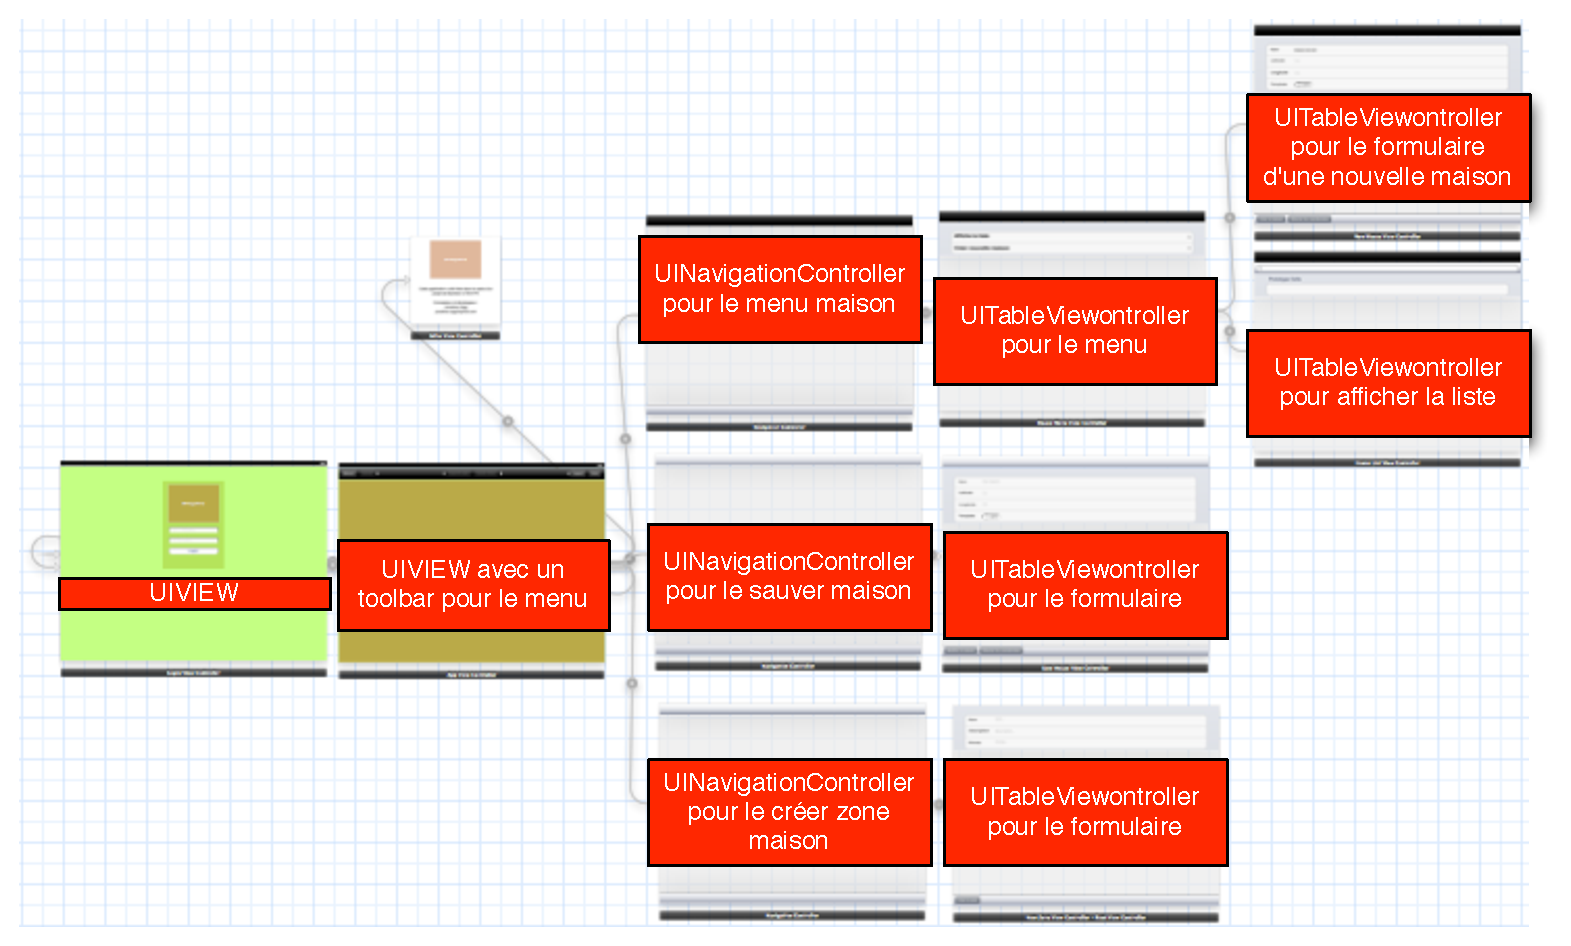
\includegraphics[angle=0,width=13 cm]{00_media/04_storyboard.pdf}
      \caption{Storyboard de l'application iGreenControl}
      \label{gra:iGreencontrolStoryboard}
\end{figure}
% subsection architecture_de_l_application (end)


\subsection{Vue logique des entités de l'application} % (fold)
\label{sub:vue_logique}

La figure \ref{gra:vueLogApp} illustre un diagramme de classes représentant les entités qui seront nécessaires à l'application. Le tableau \ref{tab:classDiagram} explique chaque entité.

\begin{figure}[H]
        \centering
        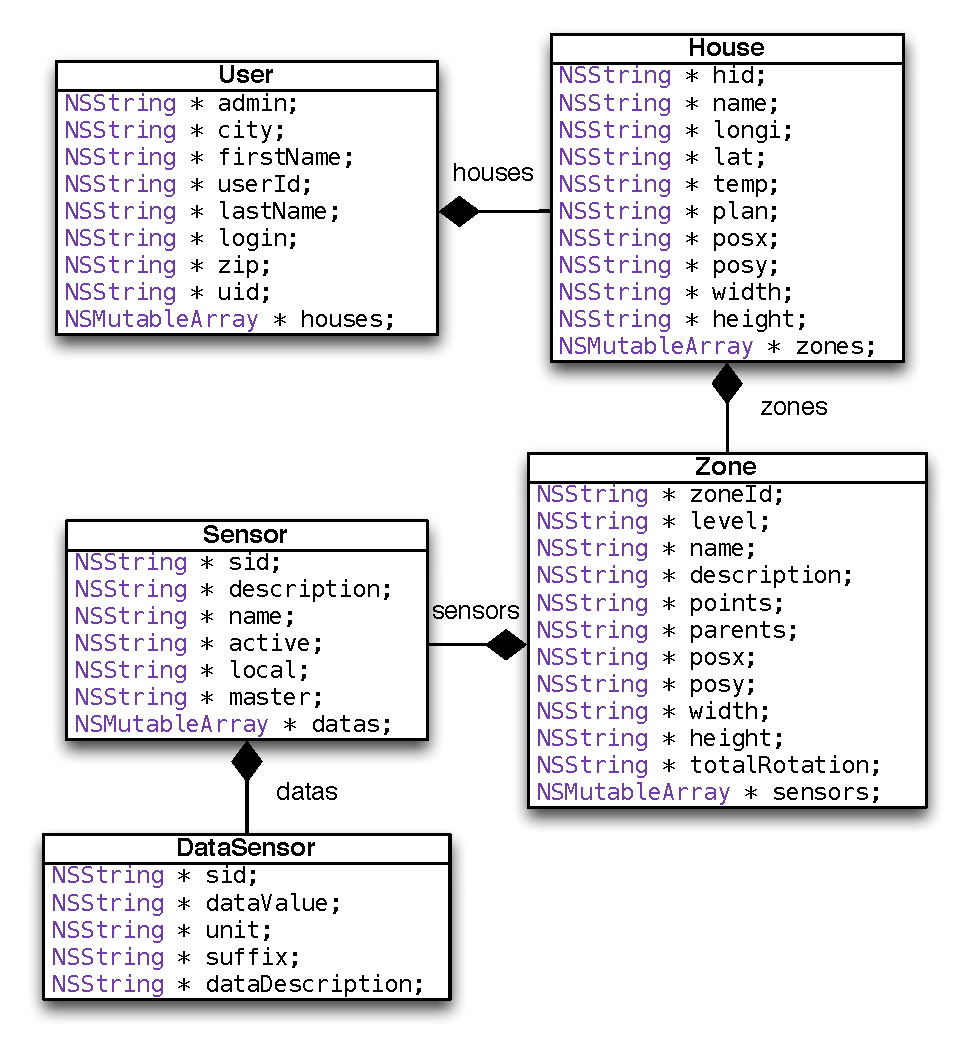
\includegraphics[width=11cm]{00_media/04_Client_Diagramme_classe_metier.pdf}
        \caption{Vue logique de l'application}
        \label{gra:vueLogApp}
\end{figure}

\begin{table}[H]
\begin{tabularx}{\textwidth}{|m{3cm}|X|l|}
  \hline
  \bf{Nom} & \bf{Description} \\
  \hline
  User & Cette entité permettra d'effectuer correctement l'authentification et de récupérer l'identification pour le bon déroulement du programme comme par exemple filtrer les maisons en affichant uniquement celles de l'utilisateur connecté. L'utilisateur disposera donc d'une liste de maison. \\
  \hline  
  House & Cette entité permettra d'effectuer des modifications sur les maisons comme par exemple en changer le nom ou l'image. Les valeurs comme width, height,  posx ou posy permettront de savoir ou positionner l'image du plan dans l'application L'entité contient également une liste de zones insérées par l'utilisateur.\\
  \hline  
  Zone & Cette entité permettra d'effectuer des modifications sur les zones insérées par l'utilisateur. Cela permettra également de savoir ou la zone est placée sur le plan et sa taille. Une zone pourra contenir des capteurs. \\
  \hline  
  Sensor & Cette entité représentera les capteurs. Elle permettra à l'utilisateur d'en changer les paramètres comme le nom, la description, etc... De plus un capteur contient des données qui sont représentées par l'entité DataSensor \\
  \hline  
  DataSensor & Cette entité représentera les données du capteurs. Plusieurs informations pourront être affichables comme par exemple la valeur, l'unité, la description, etc.. \\
  \hline
\end{tabularx}
\caption{Récapitualif du diagramme de classes}
\label{tab:classDiagram}
\end{table}

% subsection vue_logique (end)
